\documentclass[12pt,letterpaper]{report} % a4paper

% packages
\usepackage{graphicx}
\usepackage{hyperref}

% variables
\newcommand{\picSize}{0.19\textwidth}
\newcommand{\textSize}{0.79\textwidth}

% define the title
\title{Open Data Lab Annual Report - 2018}
\author{The Open Data Lab Collaboration}

%%% ---ooo000 END PREAMBLE 000ooo---

\begin{document}

% generates the title
\maketitle

% introduction
% include content
\chapter*{The Team}  \begin{tabular}[t]{lp{\textSize}}
\hline
\hline

\raisebox{-0.84\totalheight}{
\includegraphics[width=\picSize]{images/people/alonzi.png}}
& 
\begin{tabular}[t]{p{\textSize}}
$\mathbf{Pete\:Alonzi}$ came to data science by way of the particle physics community. As a result, he has great interest in making data open and usable to broad audiences. He serves as a data scientist at the DSI and is the project manager for the Open Data Lab.
\end{tabular}
\\\hline

\raisebox{-0.84\totalheight}{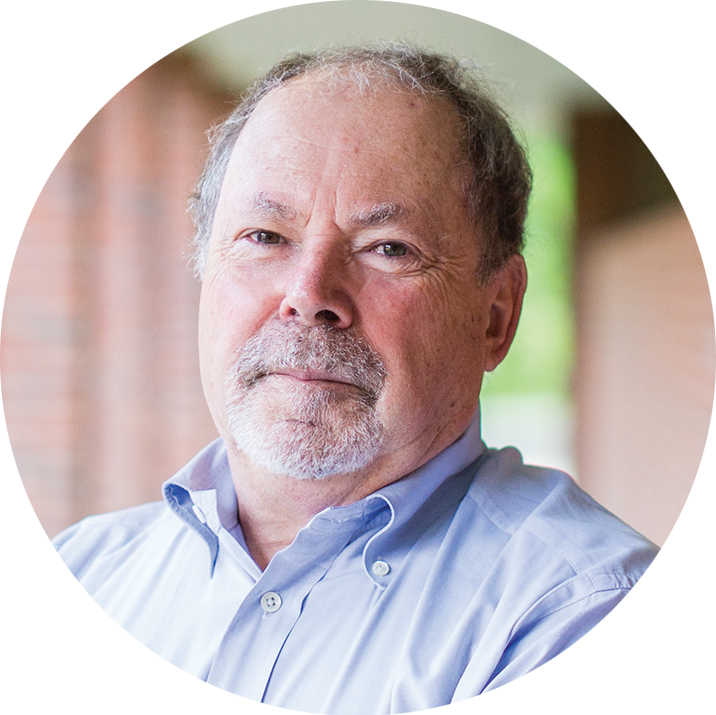
\includegraphics[width=\picSize]{images/people/bourne.png}}
 & 
 \begin{tabular}[t]{p{\textSize}}
$\mathbf{Phil\:Bourne}$ "At vero eos et accusamus et iusto odio dignissimos ducimus qui blanditiis praesentium voluptatum deleniti atque corrupti quos dolores et quas molestias excuri sint occaecati cupiditate non provident,At vero eos et accusamus et dent, " 
\end{tabular}
\\\hline

\raisebox{-0.84\totalheight}{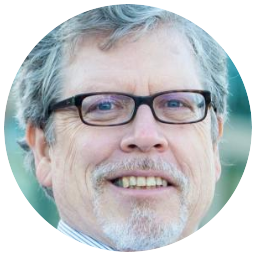
\includegraphics[width=\picSize]{images/people/clark.png}}
 & 
 \begin{tabular}[t]{p{\textSize}}
$\mathbf{Tim\:Clark}$ "Tim Clark, Ph.D., is a biomedical informatician and computer scientist with 28 years experience in academic, government and industry.  He is an expert in biomedical knowledge representation, data fusion and open science applications. He is an Associate Professor appointed in the UVA School of Medicine \& the Data Science Institute." 
\end{tabular}
\\\hline

\raisebox{-0.84\totalheight}{
\includegraphics[width=\picSize]{images/people/levinson.png}}
 & 
 \begin{tabular}[t]{p{\textSize}}
$\mathbf{Max\:Levinson}$ "Max Levinson is a  Software Engineer and Cloud Developer within Public Health Services. When not building out REST apis for the NIH Data Commons Project, he can be found hacking on the Open Data Lab Project.

Max is passionate about microservices development, knowledge graphs, and anything Python." 
\end{tabular}
\\\hline

\raisebox{-0.84\totalheight}{\includegraphics[width=\picSize]{images/people/mietchen.png}}
 & 
 \begin{tabular}[t]{p{\textSize}}
$\mathbf{Daniel\:Mietchen}$ is a data scientist at the DSI. Trained as a biophysicist, he is interested in how research can be performed openly and collaboratively across traditional boundaries like disciplines, jurisdictions, economic sectors, languages, or professional versus volunteer participants.
\end{tabular}
\\\hline

\raisebox{-0.84\totalheight}{
\includegraphics[width=\picSize]{images/people/rasberry.png}}
 & 
 \begin{tabular}[t]{p{\textSize}}
$\mathbf{Lane\:Rasberry}$ "At vero eos et accusamus et iusto odio dignissimos ducimus qui blanditiis praesentium voluptatum deleniti atque corrupti quos dolores et quas molestias excuri sint occaecati cupiditate non provident,At vero eos et accusamus et dent, " 
\end{tabular}
\\

\hline
\hline
\end{tabular}

% \smash{...} to override bounding
 % People working on project, alphabetical

\chapter*{Letter from the editor}  At the beginning of 2018 the Open Data Lab was an idea, a sketch on a whiteboard. Today the Open Data Lab has over 100 users. Students at the University of Virginia have used it to conduct research published by IEEE. In just over a year a small team of dedicated individuals from the Data Science Institute at UVA produced a product that furthered the educational and research mission of the University. Today students at UVA can do things they could not do before this project launched.

I am extremely honored to have been asked to lead this effort. The work done by our collaboration is of the very best calibre and I am proud of the work we have done and will do in the future. As project manager I feel I have the easiest job on the team. I ask everyone for ideas and they put forth not just an enormous number of ideas but also brilliant ideas. The hardest part for me is to choose from all the great ideas. Without the team Phil Bourne has built my job would be impossible. With this team I do not see any limit to what we can achieve.

The first year of the Open Data Lab was one of exploration. We discovered new tools, in particular the value of Project Jupyter. We also interviewed our potential users and recognized archetypes which we can use to guide what we build. Putting all of this together we are currently developing a strategic plan for the next three years. We now look to make an impact in the community and I am excited for what is to come.

\begin{flushright}

\bigskip

Open Data Lab Project Manager

\bigskip

Peter Alonzi

\end{flushright}
 % Mission and vision and philosophy

% insert the table of contents
\tableofcontents
\pagebreak

\chapter{Overview} \section{What is the Open Data Lab?}
\subsection*{OPEN}
We encourage all users to be as open as possible with every aspect of their work. That may be in opening up their data sets, publication, source code, or something else.
The Data Science Institute working definition of Open:
\begin{quote}
Openness means team members responsibly sharing their data and professional endeavors (when possible and ethical). We believe in the importance of practicing openness because advancement requires assembling a heap of known pieces into a coherent picture containing new knowledge. In the world today some of the necessary pieces are unknown due to traditional non-open information practices. Wide spread open practices are the first steps to changing the world.
\end{quote}

This definition was developed by the DSI open working group. Their phase one summary is listed in Appendix~\ref{chap:owg}.

\subsection*{DATA}
We take an expansive definition of data. Everything from traditional data, to code, to workflows, to published material, and so on is considered data to us. We provide a place for all things digital data.
\subsection*{LAB}
We provide a place where the power of computing can be brought to bear against data resources. Given the scale of data today this means colocating the data and computational resources.
\subsection*{Open Data Lab}
The Open Data Lab is a resource to provide state of the art computing and data infrastructure to researchers, students, and sharers. It is guided by the principles of science and openness.
 
\section{User Archetypes}
\label{sec:archetypes}
There are many potential use cases for the Open Data Lab. In this section we describe the three cases that have been studied so far. They are: the Collaborator, someone who is working on a research project; the Student, someone who is using the Open Data Lab to learn; and the Sharer, a person with data who wants to open it up to a broader audience.

\subsection*{The Collaborator}
This archetypal person uses the Open Data Lab to conduct research. They access data and computational resources that are colocated. This colocation facilitates lower latency and increased performance. A wide range of services can be provided globally by AWS and locally through UVA HPC resources. Sample workflow:
\begin{enumerate}
\item Request a user account on the Open Data Lab
\item Once per collaboration:
\begin{enumerate}
\item Load data 
\item Provision computational resources
\end{enumerate}
\item Conduct research operations
\item Register resulting products in Dataverse
\end{enumerate}

\subsection*{The Student}
This archetype uses the Open Data Lab to facilitate learning. An example would be someone who participates in a workshop where and ODL notebook instance powered by AWS SageMaker provides the working environment. Sample workflow:
\begin{enumerate}
\item Request a user account on the Open Data Lab
\item Logon to AWS console to launch Jupyter
\item Use Jupyter during the workshop
\end{enumerate}

\subsection*{The Sharer}
This archetype is a user who owns data and wants to make it available. There are many mechanisms for sharing the data ranging from RESTful API of S3, to a SPARQL endpoint. Sample workflow:
\begin{enumerate}
\item Request a user account on the Open Data Lab
\item Load data into an S3 bucket
\item Configure one of the following
\begin{enumerate}
\item SPARQL endpoint
\item API Gateway to access S3
\item S3 permissions for a SageMaker notebook
\item ...
\end{enumerate}
\end{enumerate}

\pagebreak
\section{User Summary}

\begin{table}
\begin{center}
\begin{tabular}{lccr}
\hline
\hline
group & projectID & \# members & type \\
\hline
\hline
Bourne-Mura & bamc & 4 & MSDS Capstone \\
CBW & cbwc & 4 & MSDS Capstone\\
Wiki & wiki & 10 & MSDS Capstone\\
Mental Health & miip & 6 & SYS Capstone\\
\hline
Women Terror Recruitment & watr & 2 & Presidential Fellow\\
\hline
Healthy Markets & hmtt & 5 & DSI Research\\
Independent Study & pmis & 1 & DSI Research\\
Grommullyang & & 3 & DSI Research\\
\hline
Linked Open Data   & nept & 2 & External Data\\
\hline
Spark & sprk & 17 & Education \\
GitHub & gith & 9 & Education \\
Practice of DS & 60 & Education \\ 
\hline
ORCI & orci & 2 & ODL Development\\
\hline
ML under & mlunder & 7 & Club\\
ML grad & mlgrad & 3 & Club\\
\hline
Rivanna & -- & 11 & Local\\
Ivy & -- & 6 & Local\\
\hline
\hline
ODL-education  & -- & 26 & Education Users\\
ODL-users & -- & 116 & Unique Users\\
\hline
\hline
\end{tabular}
\caption{Summary of ODL Users}
\end{center}
\end{table}

\section{A phased approach}
\label{phases}
The first three phases of the Open Data Lab have been outlined. Phase 0 focused on pre investigation and decided on what technology to test in Phase 1, the closed beta. Phase 2 is an open Beta and will serve the community of Charlottesville and other associated research and educational efforts.

\begin{table}
\begin{center}
\begin{tabular}{lccr}
\hline
\hline
Phase & type & start & end \\
\hline
0 & alpha & FEB 2018 & JUN 2018\\
1 & closed beta & JUL 2018 & MAY 2019 \\
2 & open beta & TBD & -- \\
\hline
\hline
\end{tabular}
\caption{ODL phase schedule}
\end{center}
\end{table}

To realize phase 2 we need a person to take ownership of each element of the Open Data Lab that moves into phase 2. We also require a personnel roster capable of providing service at the level necessary for the users. That requires hiring and as a results the timeline is TBD.

Put another way, the current bus factor\footnote{\url{https://en.wikipedia.org/wiki/Bus_factor}} for the open data lab is 1.

\section{What's next for the Open Data Lab?}
Starting at the end of the 2018-2019 academic cycle we have restructured the Open Data Lab Effort. We are now moving to a targeted impact strategy. What we call phase 2 (open beta) will focus on particular areas of impact. At this time the collaboration is undergoing a strategic planning effort. This effort will produce a plan to guide the Open Data Lab development over the next three years. It aligns with and inherits from the DSI plan as well as the UVA strategic plan put forth by President Ryan.


\chapter{Key Developments} This year saw great progress for the Open Data Lab. Early on there were weekly meetings to define goals and objectives. Those meetings lead to implementation of several areas and this chapter presents the key developments during 2018.

\section{Phase 1 Closed $\beta$}
The first decision made for the Open Data Lab was to implement a staged approach. Section~\ref{phases} summarizes the whole scope. This section discusses the state of the closed beta (Phase I). The user base for this phase is predominantly the Data Science Institute. There were 42 participants ranging from students, to faculty, to staff. There were also 26 workshop attendees ranging from a diverse selection of UVA researchers to community members.
The primary goal of this phase is to test different technology solutions to anticipated needs (see section~\ref{techsolu}. Those range from data storage to computation to discovery to pedagogy, and so on. Of particular note was the wild success of implementing Project Jupyter. The tools developed by this project served many roles and were excelent (details in section~\ref{projectjupyter}.
This phase will run until several criteria are met. The first is the establishment of a new funding model that will cover the scope of the open beta test. The second is the acquisition of new staff. Currently the Open Data Lab has a bus factor of one and that is not acceptable for phase 2. There are other criteria to be developed the chief of which is to scope the open beta.

\section{Establishment of User base}
This year saw the birst of the Open Data Lab and growth to include 68 users. Those users take various form from capstone research programs at the graduate and undergraduate level to full fleged dissertation research. Some of the users involved are dealing with datasets that now reside within the Open Data Lab. Currently those datasets and under tight restriction as we explore proper security protocols. There is also a contingent of undergrad and graduate students that are part of data science clubs at UVA who gain access to resources through the Open Data Lab.

It is important to understand that the technology behind the system is not the driver of the system. The needs of the user are. Right now the closed beta format allows us to interview new users and tailor a program to them. Sometimes we get the resource wrong and adjustments have to be made.
Regarding data storage the use of S3 storage from Amazon Web Services has served a broad selection of users well. Recent developments in AWS object storage technology enable users to use it as if it were block storage. As a result S3 has proved an effective solution both for large scale data storage as well as database query repositories.
Providing computational resources has been guided by the user base as well. As the base grew it became clear that the notebook technology developed by Project Jupyter was highly effective and actually resulted in more people volunteering for the closed beta test. The use of that technology helped bring users into the system.


\section{Technology Exploration}
\label{techsolu}
Many different technologies were tested in 2018. Many options using Amazon Web Services were explored and almost to a point those services were excellent. Local UVA resources were also used and in particular the UVA HPC portal developed out of the VP-IT's office is phenomenal. Collaboration is also underway with the UVA library regarding the discovery component of the Open Data Lab and the implementation of Harvard's Datavese, known locally at UVA as Libra. For version control and sharing purposed GitHub was evaluated.

\subsection{Amazon Web Services}
Cloud computing provides agility that local computational resources do not. To that end we established a contract with Amazon Web Services (AWS) through the third-party vendor DLT solutions. This contract is collectively negotiated and takes advantage of the Internet-2 network. \href{https://www.internet2.edu/products-services/cloud-services-applications/amazon-web-services/}{Here is a link to the contract details}.

In selecting a cloud resource provider our choice was informed by the needs of the  MSDS students at the DSI. The most requested cloud service was AWS and the plurality of job postings that are interested in cloud skills prefer AWS. During 2018 the initial scope of the AWS exploration was for functionality on colocating data and computation. However there was substantial mission creep and now Pete has functionally become the sysadmin for the DSI AWS account.

In the following sections we will breakdown the different services used by the ODL.

\begin{center}
Summary of Services Evaluated in 2018
\begin{tabular}{lccr}
\hline
\hline
Service & Function & Notes \\
\hline
\hline
S3 & Object Storage & \$30/TB/yr \\
EC2 & Compute Instances & \href{https://aws.amazon.com/ec2/pricing/on-demand/}{pricing} \\
SageMaker & Project Jupyter & popular interface \\
IAM &  Identity and Access Management  & users and groups \\
API Gateway & Credentialed REST & allows trigger of lambda \\
Lambda & Serverless Functions & perform miscellaneous tasks\\
CloudWatch & Log/Monitor/Alarm & more important once scaled \\
\hline
\hline
\end{tabular}
\end{center}

\subsubsection{S3}
This service provides the cheapest usable storage solution at scale. Furthermore recent policy developments at Amazon now require that other services interact with S3 (object storage) with comparable performace to block storage. That policy is very good for the ODL purposes. It means that cheaper Object Storage can be used for larger and larger datasets without yielding performance of execution. Additionally this means only one storage solution needs to be implemented. We do not need to provision additional block storage for execution operations requiring data migration and costs of duplicate storage.

The S3 systems divides the data into buckets. For this test we treated a bucket as the unit holding data for a particular research project. As a result we have 22 buckets provisioned to accomodate all of our efforts. All buckets on AWS are localized to a region but must have a globally unique name. To that end for phase 1 we have adopted the following convention. Each bucket id begins with 'odl-' and is followed by the four character project id (eg: odl-hmtt).

\begin{center}
Summary of S3 Buckets Provisioned for ODL 2018
\begin{tabular}{lccr}
\hline
\hline
ID & Project & Notes \\
\hline
\hline
odl-bamc & Bourne/Mura Capstone & \\
odl-bamc-scratch & Bourne/Mura Capstone & scratch space \\
odl-cbwc & & \\
odl-dome & Dominion Capstone & defunct \\
odl-hmtt & Healthy Markets & 13\,TB \\
odl-hmtt-scratch & Healthy Markets & scratch space \\
odl-nept & Numismatic Linked Open Data & in development \\
odl-orci & Educational Open Datasets & in development \\
odl-pmis & & \\
odl-podc & DSI Communications & \\
odl-projhects-test & DSI project configurations & \\
odl-readonly-test & read only test & \\
odl-scratch-test & scratch space test & \\
odl-sp19-sys6016 & Class materials & \\
odl-spark-education & Spark Educational Materials & \\
odl-spark19spds6003-001 & Class Materials & \\
odl-watr & Women and Terrorism Recruitment & \\
odl-watr-scratch & Women and Terrorism Recruitment & \\
odl-wiki & Wiki Capstone & \\
\hline
2017-2018-capstone-plos & 17/18 capstone & remnant from phase 0 \\
uva-bucket & initial test bucket & remnant from phase 0 \\
846033058400-dlt-utilization & DLT bucket & part of DLT contract \\
\hline
\hline
\end{tabular}
\end{center}

For the example of 'odl-hmtt' this bucket serves the Healthy Markets project. We bill that project PTAO for the service the ODL provides. The mechanism is to pay the DLT contract off the ODL PTAO and then do a cost transfer annually from the Healthy Markets PTAO to the ODL PTAO.

\subsubsection{13\,TB Data Transfer}
When we acquired the Healthy Markets dataset we transferred it from their aws bucket to ours. However this transfer was not trivial. AWS was unwilling to change the bucket ownership from their account to our so we had to copy the data over.

The recommendation was to use the AWS CLI to perform the copy. It functions very similarly to scp from standtard unix systems. However we discovered several interesting features.
\begin{itemize}
\item Some of the files were copied to our bucket using an IAM account on their AWS account. Then Healthy Markets deleted that IAM user and as a result we lost control of the files in our bucket. Efforts to regain control are ongoing through DLT solutions.
\item Direct bucket to bucket transfer is managed via a serverless operation and does not prototype the transfer. As a result the resources allocated automatically were not sufficient to transfer 13\,TB during a human lifetime. We then setup a dedicated server via EC2 and were able to configure the system to complete the transfer at a rate of about 4\,TB per day. We did incur cost for operating that server but is was not prohibitive.
\item The AWS CLI is not optimized for mass transfer and to copy the data in a reasonable timescale we had to write some scripts to chunk the operation. That work is located on the \href{https://github.com/UVA-DSI/Open-Data-Lab/tree/master/aws/large_s3_transfer}{ODL github page}.
\end{itemize}

\subsubsection{EC2}
This service allows for provisioning of compute resources. We established lambda functions to automate the create of EC2 instances for projects given a json configurationf file. Here is \href{https://github.com/UVA-DSI/Open-Data-Lab/blob/master/aws/lambda/src/stand_up.py}{the link to the code}. And here is a sample JSON file:

\begin{verbatim}
{
   "projectId": "open-data-lab",
   "github": "https://github.com/UVA-DSI/Open-Data-Lab.git",
   "data-bucket": "odl-hmtt",
   "scratch-bucket": "odl-scratch-test",
   "ImageId": "ami-b70554c8",
   "InstanceType": "t2.nano",
   "email": "lpa2a@virginia.edu",
   "maxNumInstances": "1"
}
\end{verbatim}

These EC2 units are monitored by the CloudWatch system and we can configure them to turn on and off as necessary.

The majority of our users use EC2 as their compute engine however they access the compute via auto-provisioning from the SageMaker service.


\subsubsection{SageMaker (Project Jupyter)}
\label{projectjupyter}

SageMaker has been the breakout star of the 2018 ODL development phase. Our MSDS students prefer Project Jupyter as their mechanism for using computational and storage resources. To that end Pete went to the JupyterCon in New York City in the fall of 2018. \href{https://github.com/UVA-DSI/conferences/tree/master/JupyterCon18}{Details of his experience are found here}.
At this conference Pete was able to speak directly with the creators, developers, and users of Project Jupyter as well as the AWS developers of SageMaker. This service through the power of Project Jupyter is able to democratize the access and management of computational resources. The systems lifts a large cognative load off the user and empowers them to accomplish their goals efficiently without requiring arcane knowledge of computers. Our working metaphor is as follows:

\begin{quote}
\textbf{
The user is able to drive the car and get where they want to go without needing to first learn how to build a transmission.
}
\end{quote}

This power is the true killer feature of Project Jupyter and is the reason the system is so popular and widely used. Often people we say the ability to break code into cells and use markdown and inline plotting is the killer feature but it is really the lifting of the cognitive load.

\subsubsection{IAM}
This services governs Identity and Access Management. It breaks down into users and groups. Users are placed into appropriate logical groups and then access policies are assigned to groups.
When testing permission settings a dummy IAM user is established and given the same groups as the user being tested. In that way the sysadmin can see what the user sees and debug/test/prepare the system to the user.
\subsubsection{API Gateway}
We configured an API gateway to provide a mechanism for the users to trigger lambda functions. The users require credentialing via the standard aws authentication protocol when the post to the Gateway. \href{https://github.com/UVA-DSI/Open-Data-Lab/blob/master/aws/api-gateway/hitapi.py}{Details of the system are on the GitHub here}.
\begin{verbatim}
requests.post('https://pish6mpnr0.execute-api.us-east-1.amazonaws.com/alpha-2/vm_stand_up',
                        auth=auth,
                        params={'projectID':sys.argv[1]})
\end{verbatim}



\subsubsection{lambda}
This services allows for serverless execution of code. Currently we use it for provisioning of EC2 instances and automation of EC2 management.


\subsubsection{CloudWatch}
This service is how we monitor the system and record logs.

\subsubsection{Architecture Diagrams}


\begin{figure}[!hbtp]
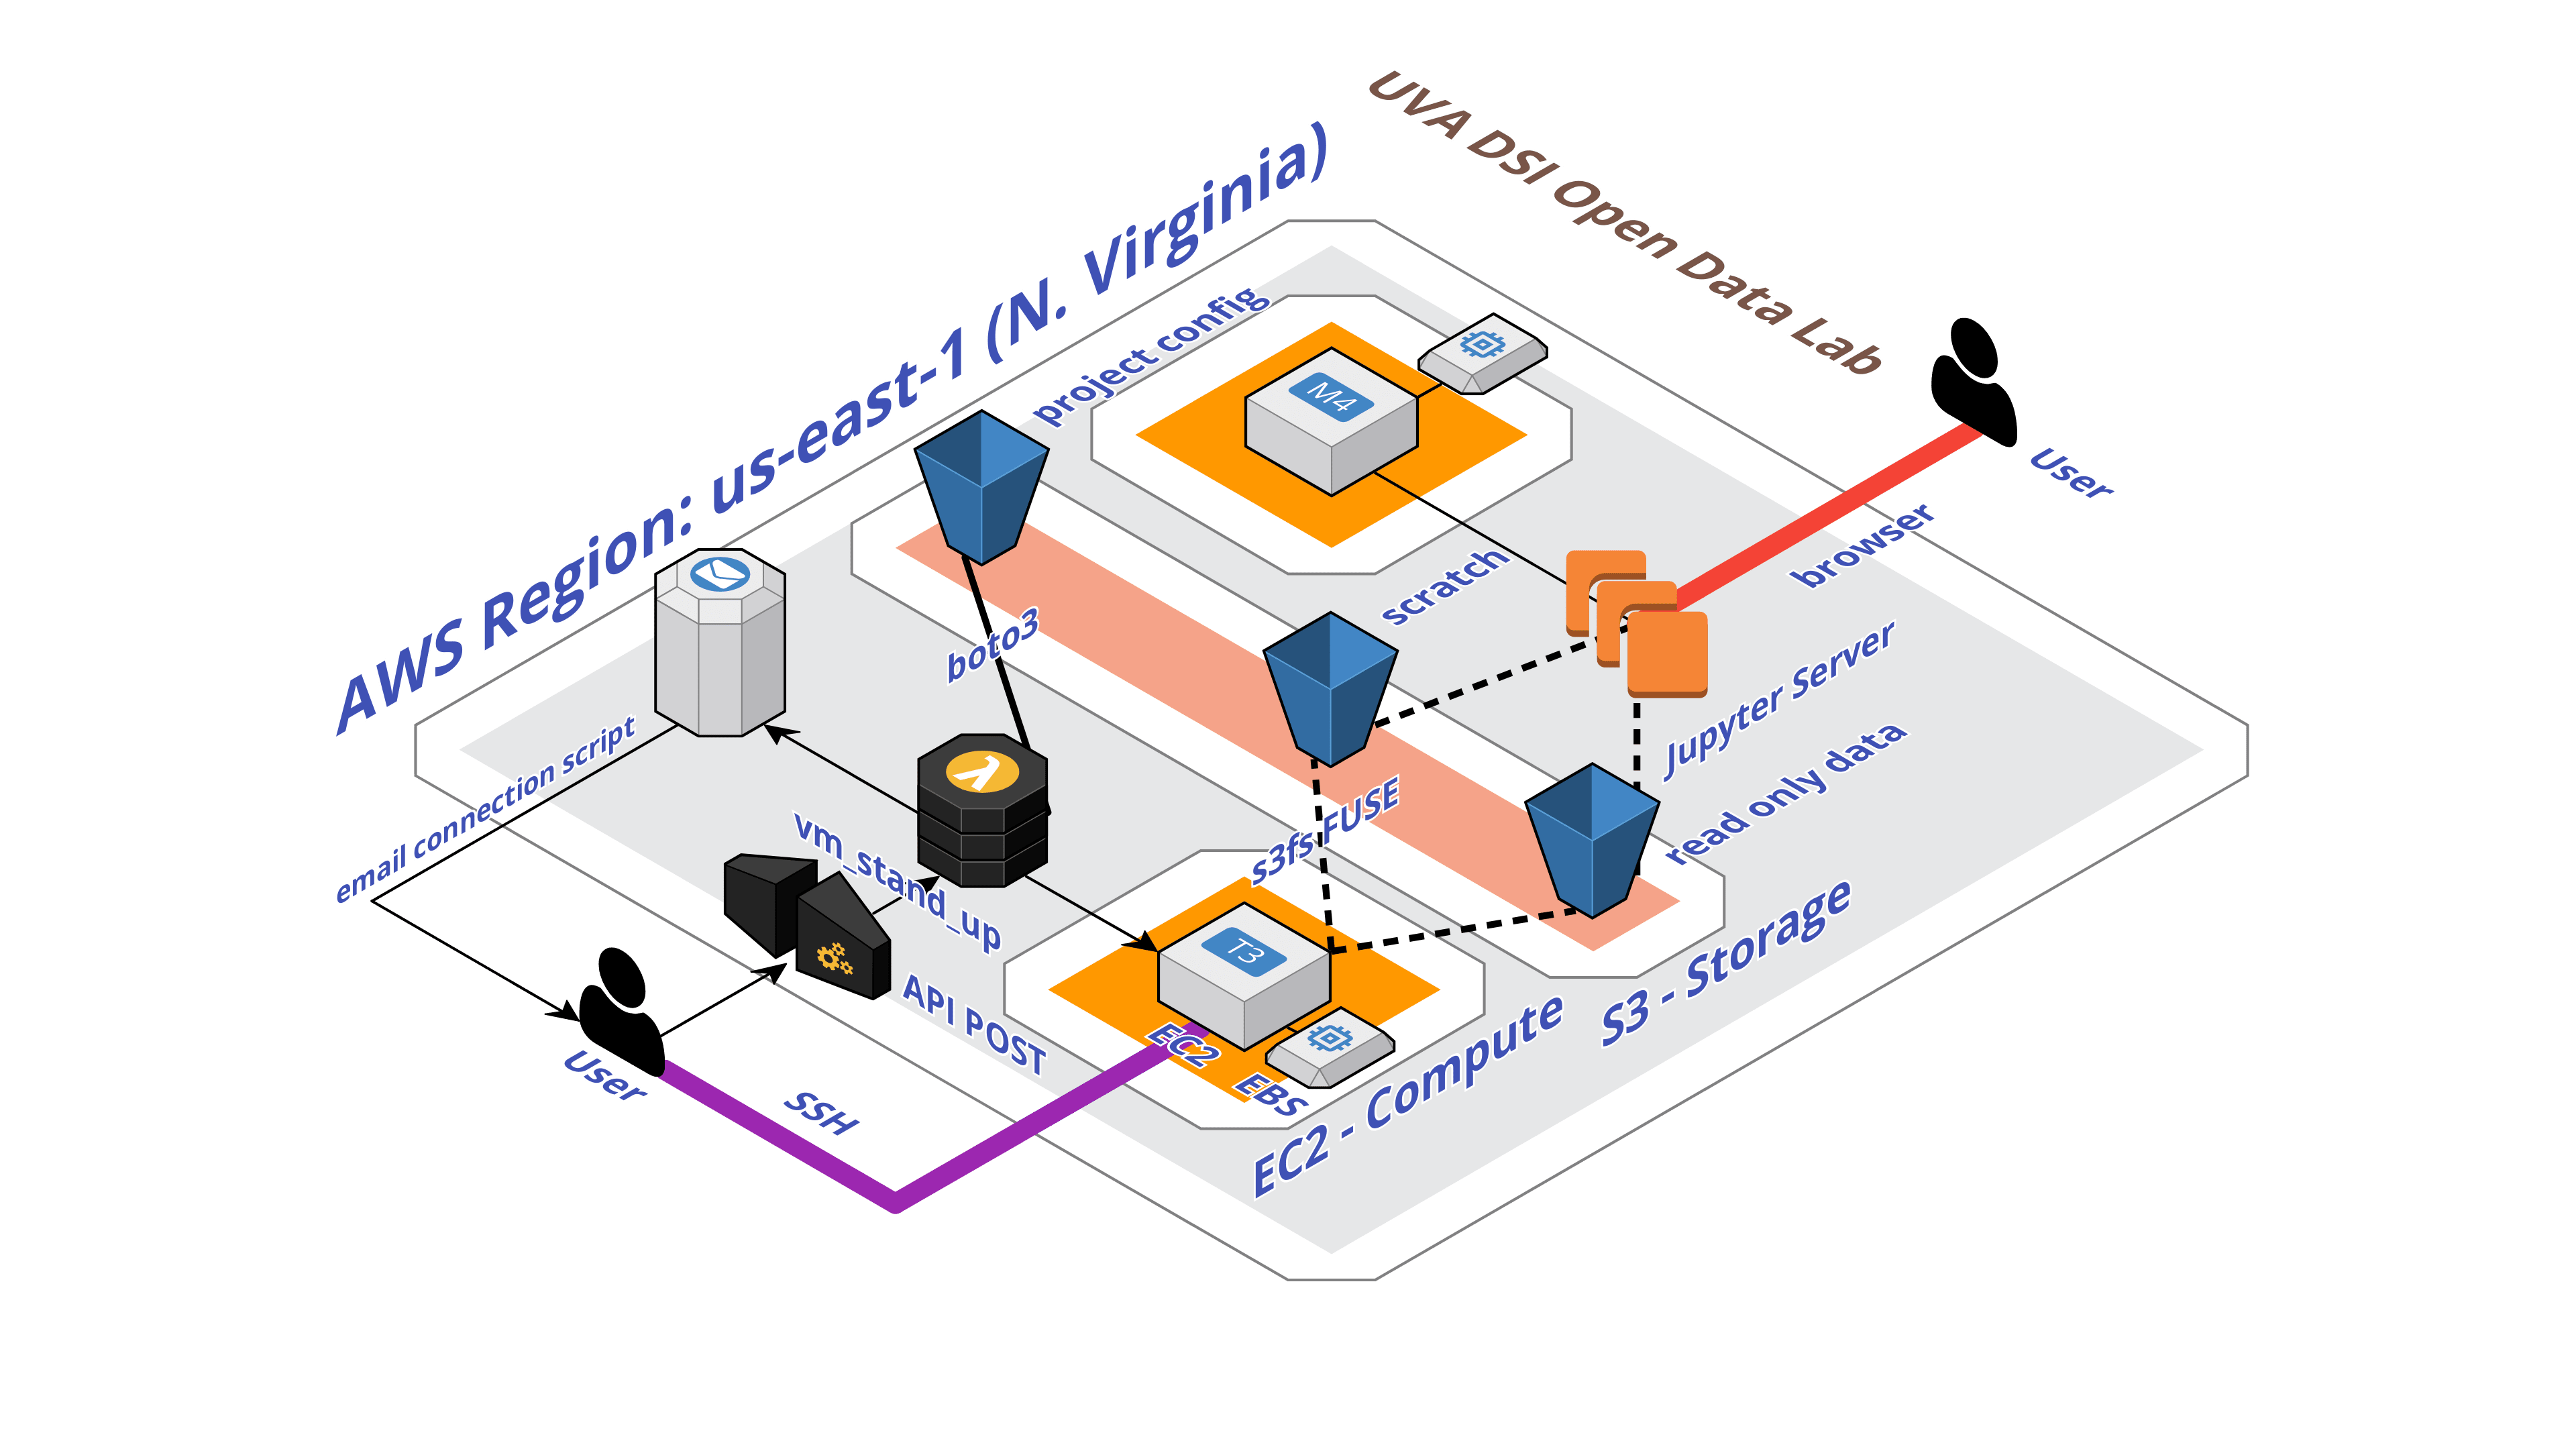
\includegraphics[width=\textwidth]{images/odl-diagram.png}
\caption{Schematic of AWS service  configuration\label{fg:aws}}
\end{figure}
\begin{figure}[!hbtp]
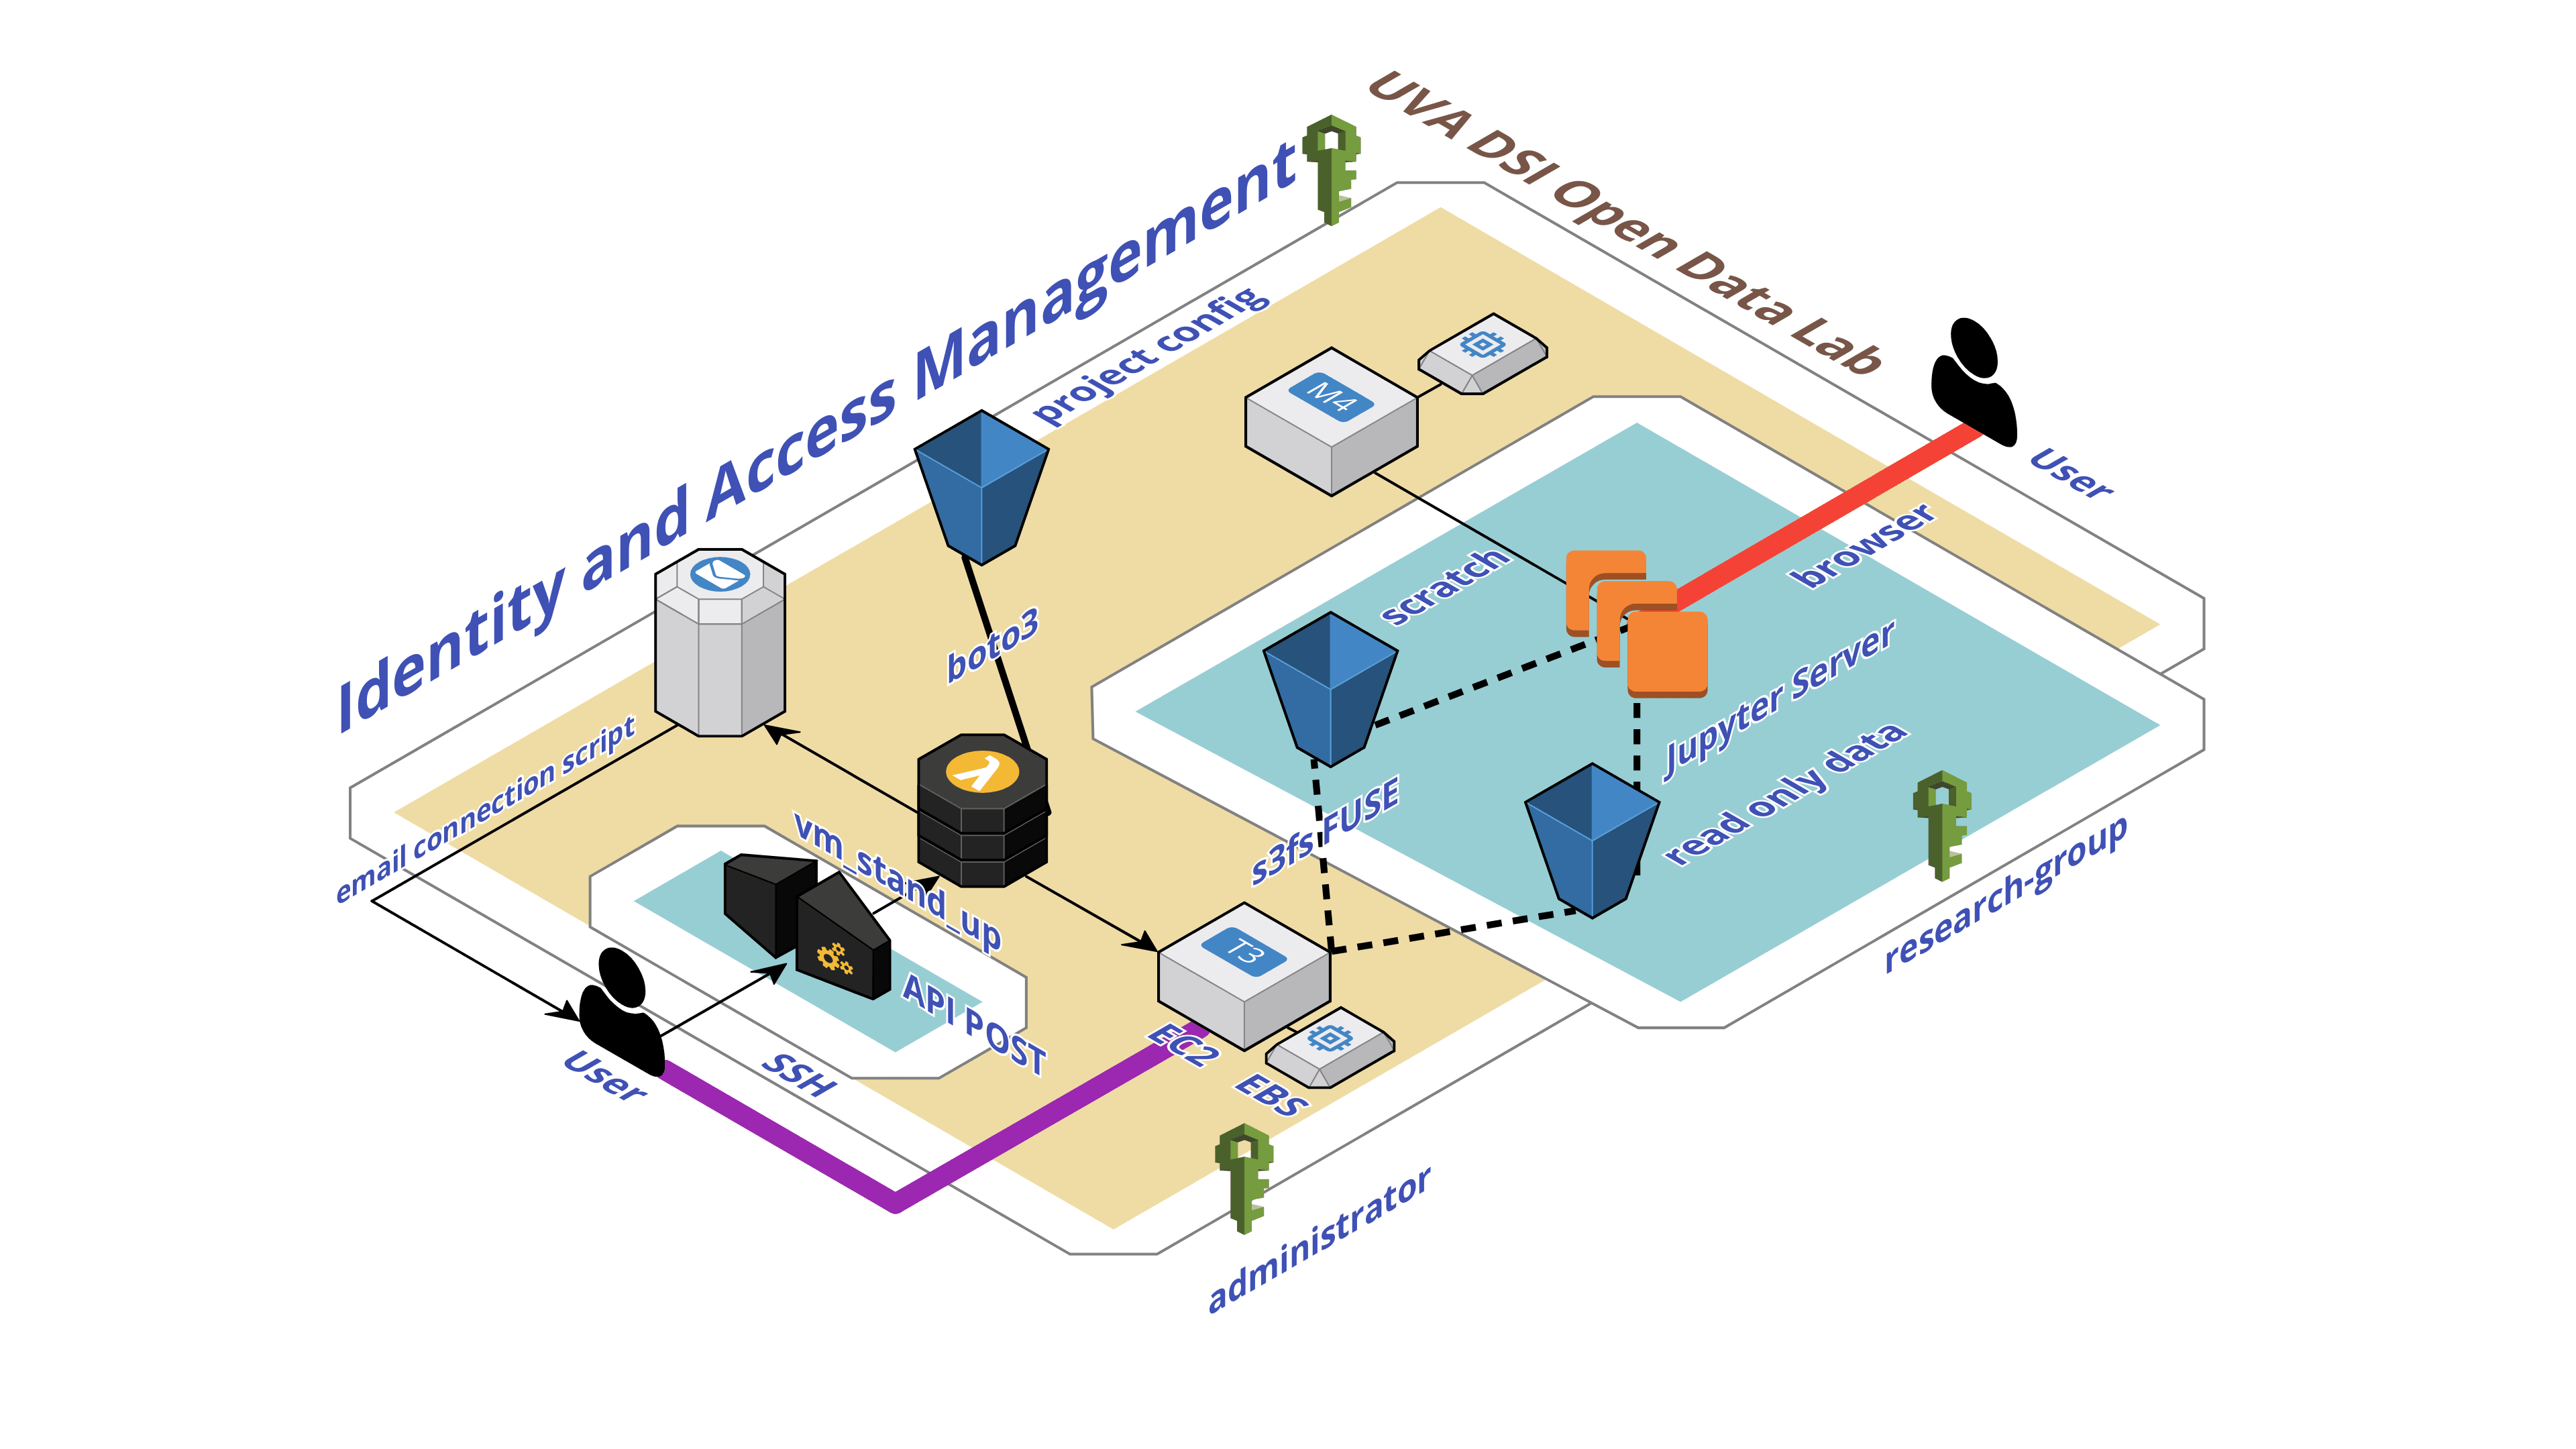
\includegraphics[width=\textwidth]{images/odl-iam.png}
\caption{AWS IAM configuration\label{fg:iam}}
\end{figure}



\subsubsection{Support Plan}
For the first year of the ODL we elected to keep the business support plan. In the future we can have a ten percent savings by eliminating this support.
\begin{verbatim}
https://aws.amazon.com/premiumsupport/compare-plans/
\end{verbatim}

\subsection{Local UVA - Rivanna and Ivy}
The local computational resources at UVA are facilitated through the office of Vice President for IT. That group is dedicated and hard working and provides great resources to the local UVA community. We have established a working relationship with them and discuss technical problems and solutions. Independently we arrived at the utility of Project Jupyter.
These solutions are for UVA personnel and their collaborators and as such will not scale to later phases of the Open Data Lab project. However for the closed and open beta it is a great resource. Furthermore their technical expertise will be invaluable to the Open Data Lab regardless of phase.

\subsection{GitHub}
GitHub is the most broadly adopted cloud platform for version control. Therefore we evaluated it first. The utility for managing repositories is fully mature. The collaborative features focused around the fork and pull request paradigm are excellent. GitHub also has project level capability with issue tracking and team/permission functionality for managing permissions and progress. We have been extremely pleased with the capabilities of GitHub. The only motivation to try other solutions is for the sake of due diligence.

Concerning the acquisition by Microsoft: Many have raised the issue that GitHub may not be the appropriate solution now that Microsoft has acquired GitHub. However the recent track record of Microsoft is to not meddle with projects like GitHub but rather to protect them. Additionally most users use other Microsoft products. What's more the Open Data Lab also relies heavily on Amazon.

\section{Upcoming Technical Exploration}
The following sections describe exploratory work that is on the schedule. There is more to be done beyond this list but not scheduled.
\subsection{Dataverse}
A framework has been outlined to use Dataverse as the discovery mechanism for the Open Data Lab. In this system a metadata entry will be made in the Dataverse containing all of the usual materials. However the final piece with the datafiles will contain pointers to the data and projects within the Open Data Lab. Dataverse is not configured for colocating computation resources with the data resources. The pilot of this test will be with the Libra project from the UVA Library. Currently that system is undergoing an upgrade and once there is a stable release exploration will commence.
\subsection{Spark}
The first scale data solution the Open Data Lab will explore is Spark. Preliminary work so far as been the development of a introductory workshop on the technology (available on the Open Data Lab github repository). A second pedagogical series will be presented early in 2019 and will lead to testing different technical solutions.
\subsection{SPARQL Endpoint}
The numismatic dataset will be accessible through a SPARQL endpoint. This exploration is in the early stage and has not matured to the point of evaluation. The next annual report will have a full breakdown of the best way to treat this form of data and delivery.


\chapter{Research} This section of the report includes excerpts from research publications produced by groups using the open data lab. We highlight a couple MSDS capstone projects (\ref{sec:BMC} and \ref{sec:wik}) as well as a faculty research project (\ref{sec:hmt}) and the undergraduate machine learning club (\ref{sec:mlc}).

\pagebreak
\section{Bourne/Mura Capstone}
\label{sec:BMC}

\emph{Sean Mullane, Ruoyan Chen, Sri Vaishnavi Vemulapalli, Eli J. Draizen, Ke Wang, Cameron Mura, asnd Philip E. Bourne}
\bigskip

The biological function of a protein stems from its 3D structure. Understanding these functions is important in biomedical research. Given the high costs of using experimental means to determine protein structures, current methods do not scale. As a result, many have attempted to apply machine learning to this problem to predict structure from amino acid sequence data.

Our work focuses on a sub-problem of this field: predicting locations of the capping motifs which terminate $\alpha$-helix protein structures. These motifs have only been described empirically to date~\cite{ref:bmc}. As a step toward a robust and statistically-based understanding of helix capping, we demonstrate that machine learning modules can be trained to predict helix cap positions from sequence data.

\begin{figure}[!hbtp]
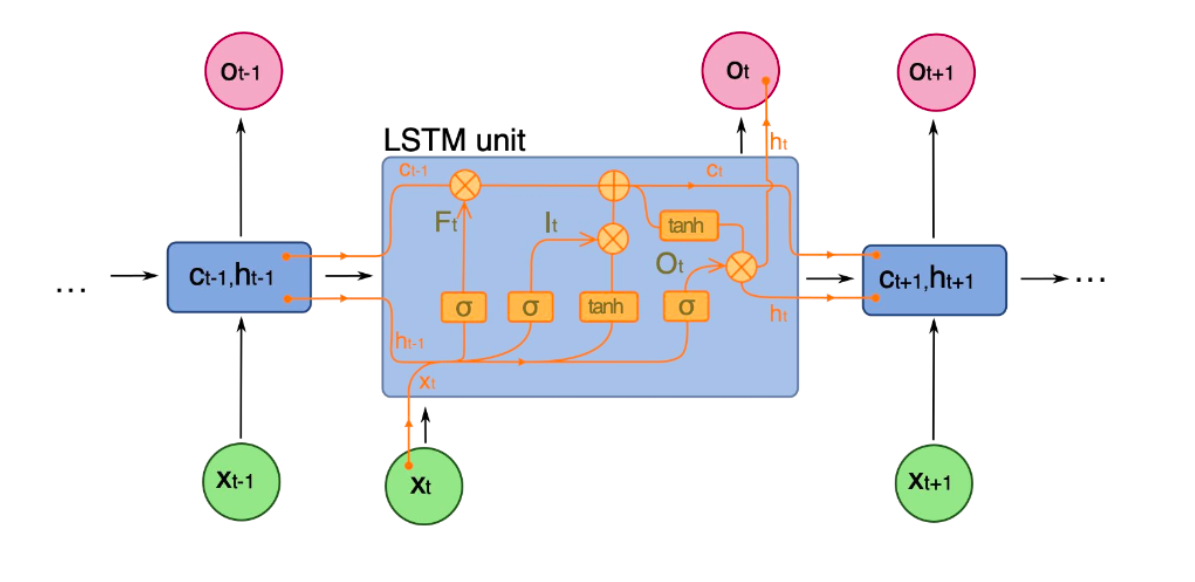
\includegraphics[width=\textwidth]{images/bmc1}
\caption[LSTM diagram]{LSTM with feature vector of single amino acid residue as input to each cell}
\end{figure}

\begin{figure}[!hbtp]
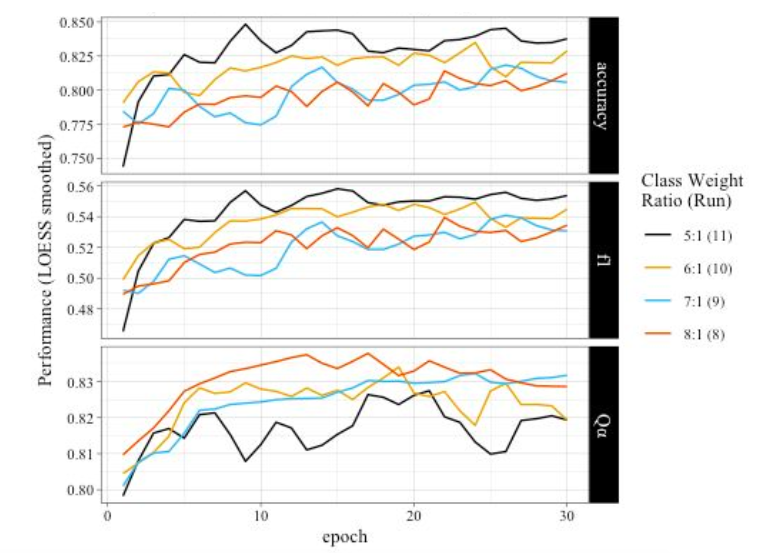
\includegraphics[width=\textwidth]{images/bmc2}
\caption[Loss function analysis]{Effect of Loss Function Weighting}
\end{figure}



From poster presented at SIEDS 2019.

\pagebreak
\section{DSI Wiki Capstone}
\label{sec:wik}

\emph{Charu Rawat, Arnab Sarkar, Sameer Singh, Rafael Alvarado, and Lane Rasberry}
\bigskip

In this paper, we propose a framework to understand and detect abuse in the English Wikipedia community. We analyze multiple publicly available data sources provided by Wikipedia. We propose a web scraping methodology to extract user-level data and perform extensive exploratory data analysis to understand the characteristics of users who have been blocked for abusive behavior in the past.

We further build upon these insights to develop an abuse detection model that leverages Natural Language Processing techniques, such as character and word n-grams, sentiment analysis, and topic modeling, to generate features that are used as inputs in a model based on machine learning algorithms to predict abusive behavior.

\begin{figure}[!hbtp]
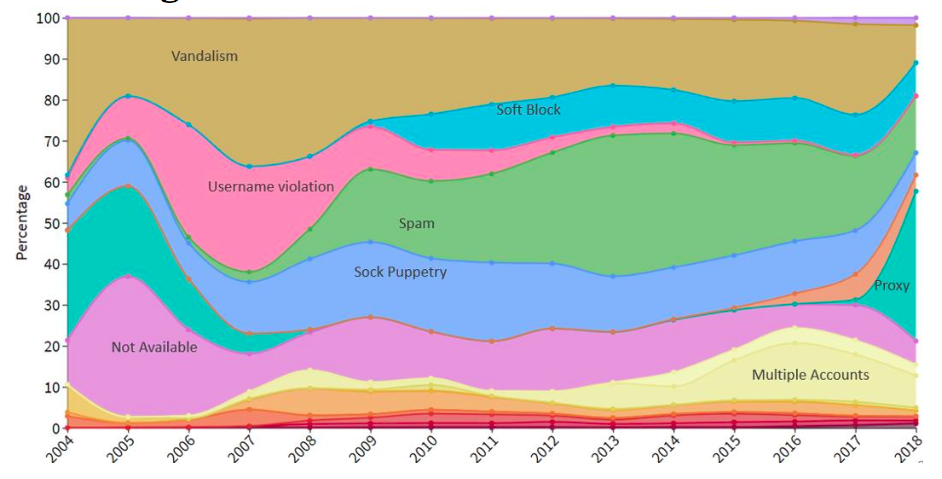
\includegraphics[width=\textwidth]{images/wiki1}
\caption[Wikipedia user blocking summary]{Share of block reasons over time}
\end{figure}

\begin{figure}[!hbtp]
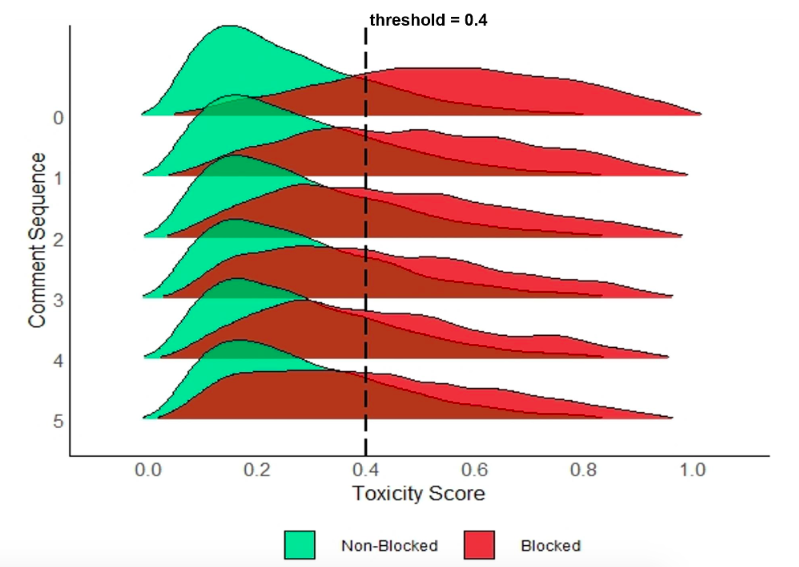
\includegraphics[width=\textwidth]{images/wiki2}
\caption{Toxicity score evaluation}
\end{figure}

From poster presented at SIEDS 2019.

\pagebreak
\section{Healthy Markets}
\label{sec:hmt}

\emph{Narges Tabari}
\bigskip

In Healthy Market project, our goal is to understand the effect of high frequency trading on variables such as social media, stock market, retirement plans, and unemployment rate. To do this, we improved the structure of multiple causal models. Examples include: 
\begin{itemize}
\item Identifying trends in high frequency trading with structural causal models that were improved by treating the time-series data as images and leveraging the power of convolutional neural networks (CNNs). We use time series data encoded as images using Gramian Angular Fields (GAF) in a classification task. We then built a structural causal model, based on the architecture of the model, that learn structural equations using CNN filter values (Shown in figure~\ref{fig:hm}). By doing this, we are able to visually present the important patterns that the model looks for in the image that can potentially be interpreted as variations in the time-series data.
\item Improving the construction and interpretability of Granger causal models with long short term memory networks (LSTMs) and hierarchical lasso penalties to find out the granger causal nature and the time lag selection between stocks of different companies 
\end{itemize}

\pagebreak
\begin{figure}[!hbtp]
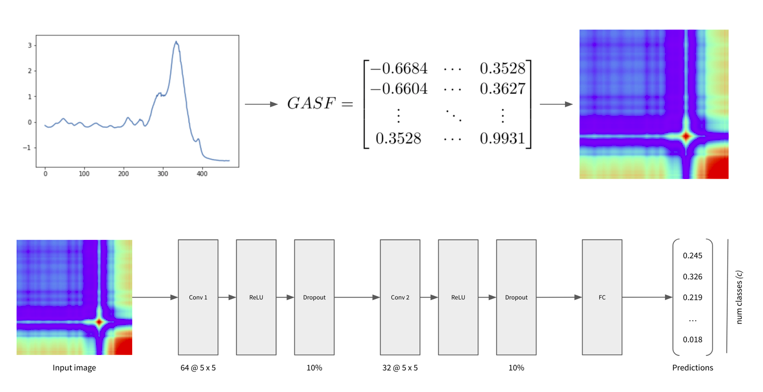
\includegraphics[width=\textwidth]{images/hm}
\caption[Healthy Markets CNN filter schematic]{Schematic of CNN filter process}
\label{fig:hm}
\end{figure}

\pagebreak
\section{Undergraduate Machine Learning Club}
\label{sec:mlc}

\emph{Jake Grigsby, James Hanson, Hugh Jones, John Morris, Jonah Weissman, Zabihullah Yousuf}
\bigskip


This semester, the Undergrad ML group built the foundations of a new Deep Reinforcement Learning platform. At its center is an implementation of Proximal Policy Optimization with Random Network Distillation. This technique, first published by OpenAI in late 2018, augments the PPO learning algorithm with the 'curiosity' to find novel states - greatly increasing performance in environments with sparse rewards by giving the agent continuous intrinsic ones. Our version is currently geared towards vision-based video game tasks; so far it supports any pixels-only environment from both Gym and Gym-Retro, but can be modified to work with any similar RL package. While the original paper came with an open source implementation, our version is more general purpose and written in TensorFlow's eager execution mode, which will make it easier to extend, debug and maintain going forward. It is also very scalable: we use synchronous gradient descent to process small amounts of data (a single rollout) on each worker, which eliminates the need for a GPU and lets us take full advantage of CPU clusters.

So far we have primarily tested the agent on Sonic The Hedgehog. While not as difficult an exploration environment as famous benchmarks like Montezuma's Revenge, Sonic is an interesting problem because of its very inconsistent difficulty. Long stretches of running right and jumping are broken up by obstacles that require significant long-term planning, creating bottlenecks that tend to destabilize training and require the agent to try new strategies over and over again. Our agent performs surprisingly well, even with just a few parallel workers. Figure~\ref{fig:mlunder} is an example chart of the training process, which shows the map and the agent's deaths, as well as the internal and external rewards.

\begin{figure}[!hbtp]
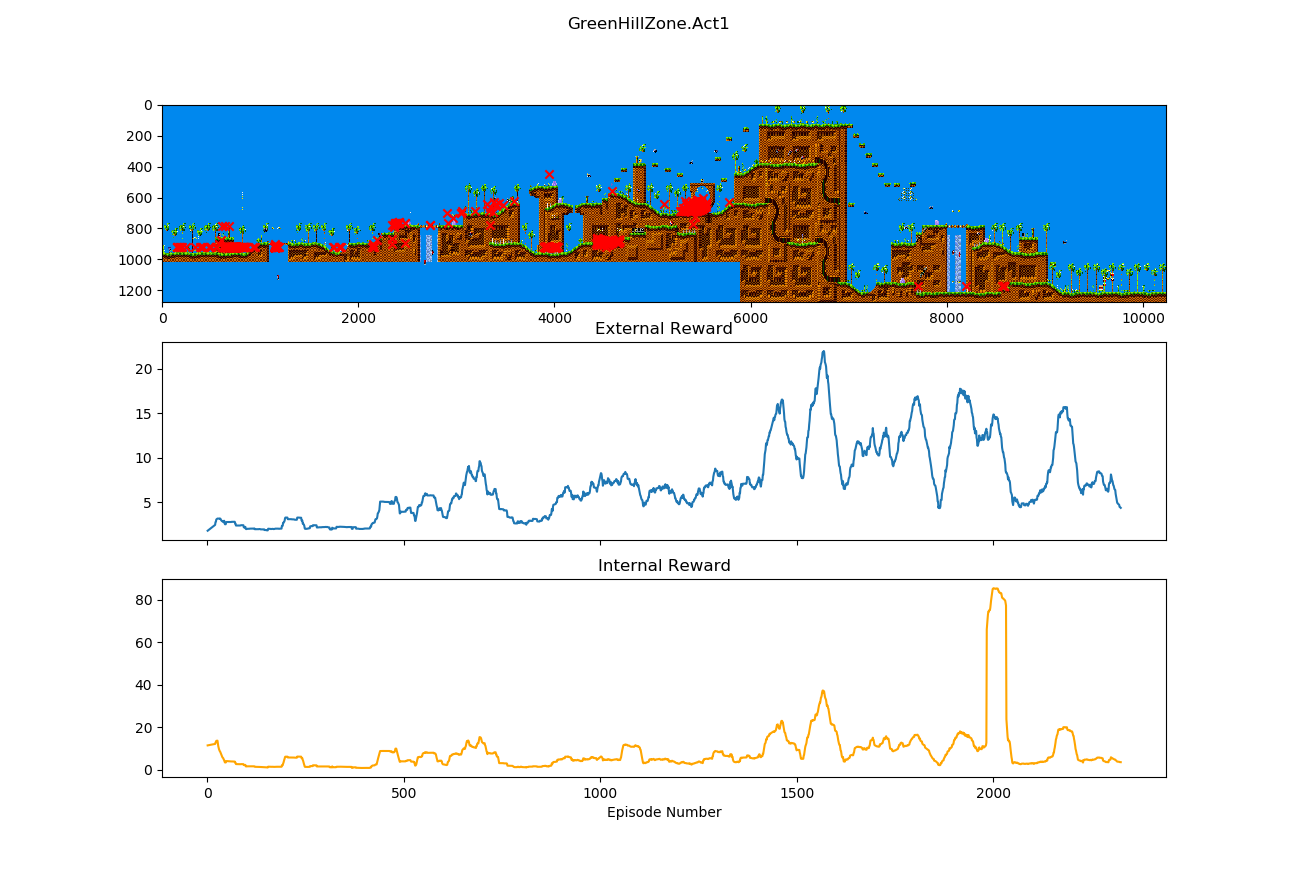
\includegraphics[width=\textwidth]{images/mlunder_figure.png}
\caption[Deep Reinforcement Learning rewards]{Example training process including rewards}
\label{fig:mlunder}
\end{figure}


%Proximal Policy Optimization with Random Network Distillation  -- https://arxiv.org/abs/1810.12894





\chapter{Education} A key component of openness is making resources usable. This idea falls in line with the idea that openness and accessibility are part of the same mission. As a result the educational component of the Open Data Lab is vital to the suces of the project. There are two main thrusts in this endeavor. The first, which was piloted in 2018, is the production of educational materials and methods. The second part is the development of communication paradigms.
This year two workshops were produced and delivered as part of the closed beta test. The first focused on the scale data protocol spark and the second the version control tool GitHub.

\section{Spark Workshop}
This workshop was designed as an introduction to spark. The goals were:
\begin{itemize}
\item Teach how to get started
\item Build comfort
\item Teach how to get answers to further questions
\end{itemize}
The topics covered included linking to a spark context, reading in data via dataframes, manipulating the data, and making a fundamental calculation.
To power the workshop the attendees were given credentials on a Amazon SageMaker notebook. One of the features of this approach is that the whole workshop has access to the same environment. Everyone sees the same implementation of the software and hardware. There is no cumbersome overhead in getting set up. The requirements are a web browser and access to the internet.
Furthermore the single notebook environment leads to a very useful pedagocial capability. When a student encounters and error in their code the instructor can load their notebook on the main display in the room. In real time and in full view of everyone the instructor can debug and teach the whole class. This is a vast improvement over the current popular method of hovering over a single learners station. It enables every person in the room to see what is going on and maintain their level of engagement. This experience was very positive for the learners and the feedback to this approach was superlative.
Previous versions of spark training was done with Databricks resources and there were several drawbacks precipitating the switch to Amazon.
\begin{itemize}
\item The environment is not shared between the workshop participants and the instructor
\item Every learner independently established their own cluster and there is substantial lag
\item Materials must be imported in Databricks format (.dbc) instead of more universal jupyter notebook format (.ipynb).
\end{itemize}

Resources:
\begin{itemize}
\item Databricks based workshop can be found at: https://github.com/alonzi/spark
\item Amazon Sakemaker based workshop can be found at: https://github.com/alonzi/spark-intro
\item Next generation materials will be incorporated into the Open Data Lab repository at: https://github.com/UVA-DSI/Open-Data-Lab/tree/master/education
\end{itemize}

The cost to operate and instructional environment is \$0.0464 per hour. For this workshop we ran the environment for one week at a cost of approximately \$10.

\section{GitHub Workshop}
\label{sec:git}
The Open Data Lab was invited to present GitHub to the Archaeology Department of the Thomas Jefferson Foundation (aka Monticello). We developed a workshop to explain the fundamentals of version control and present a work-flow for beginning users. The different user archetypes were also discussed.
One of the major burdens to version control use is that it comes from the computer superuser community. Most of the software is developed using a terminal based interlace (CLI). However in today's research world many one computer superusers interact with code and other materials that benefit from a version control workflow.
The major benefit from GitHub is the browser based interface. This implementation shifts substantial pieces of cognative load off the user. This shift enables the user to focus on developing their work rather than on the bookkeeping of version controling their work. At the same time it makes it easy for the developers to take advantage of the version control benefits.
There is substantial room to further develop materials for different user archeytypes. This workshop focused on a research group. We will strive to identify other archetypes and develop materials to suit those needs.
This workshop was taught straight from the GitHub repository itself. That was a natural fit given the subject matter. But it also demonstrated several very useful pieces of GitHub as a teaching medium, which will be discussed in~\ref{githubforteaching}.

Resources: https://github.com/UVA-DSI/Open-Data-Lab/tree/master/education/GitHub

\section{Using GitHub as a Teaching Medium}
\label{githubforteaching}
Both of the workshops taught under the Open Data Lab project used GitHub as the repository for materials. This has several benefits.
\begin{itemize}
\item GitHub provides a URL and free hosting for resources
\item Subsequent changes to the materials are stored under version control thus allowing the actual materials presented to be recovered
\item Any learner who wants to suggest improvements to materials can implement a pull request
\end{itemize}

The decision to put the materials in GitHub was one of necessity since the Open Data Lab GitHub page serves as the repository for all Open Data Lab resources. GitHub by default provides a URL for every item stored in the repository and presents the README file of a repo. This presentation is automatically rendered from markdown. Wikipedia has demonstrated the success of using markdown for content presentation but to enumerate some key features here. The document is organized, hyperlinkable, figures are easily embeded, and it seamlessly renders text alongside code and mathematical formulae.

\section{Plans for 2020}
The plans for the future of Open Data Lab education efforts are part of the upcoming strategic plan. The educational component runs across all goals. As we finalize the areas in which to make an impact educational tools will be developed to support those efforts. Most likely this will take the form of content on github and workshop materials.

\chapter{Data sets} The Open Data Lab is in the business of hosting data sets with various levels of openness. We encourage all users to make their data as open as practicable. Currently there is a purchased data set that goes by the codename 'Healthy Markets' in the ODL (it contains financial information). And we are bringing a Numismatic data set online. There are also various data sets for student research  projects hosted on the open data lab.

At the end of 2018 the total amount of data in the lab was  13.6\,TB. This is predominantly from the Healthy Markets Dataset.




\section{Healthy Markets}
The Healthy Markets dataset was purchased by the University under liscense for use by  all members of the university. The Open Data Lab is responsible for storage and providing access to the dataset. Narjessadat Seyeditabari (Narges Tabari) is responsible for facilitating research on the dataset and is the primary user of the dataset.

The data set is 13\,TB and is stored in an S3 bucket named 'odl-hmtt'. This bucket is private to users of the Open Data Lab and is accessed through a SageMaker instance. To copy the data from it's source at Healthy Markets we used the AWS CLI and it took several days with a total cost of \$1 for REST actions and \$17 for the EC2 instance to manage the transfer. The current cost to store the data set is \$290 per month. These costs are covered by the Healthy Markets PTAO.

Section~\ref{sec:hm} contains the report on research activities with this data set.

\section{Numismatic}
Dr. Ethan Gruber from the American Numismatic Society is in possession of a Linked Data Set  and wants to make it open with the Open Data Lab. He is interested in establishing a SPARQL endpoint for the  dataset. An S3 bucket (odl-nept) has been provisioned to store the data for the project and we will be making the data set open in  2019.

\chapter{Financial Report} \section{Budget} % income and outlays
The budget for the first year of the open data lab has a scope consisting of a purchase order for AWS time and personnel detailed from the Data Science Institute.

\begin{center}
Table of Income and Outlays for 2018-2019

\begin{tabular}{lccr}
\hline
\hline
Source & Time (FTE) & Time (hours) & USD \\
\hline
\multicolumn{4}{c}{Income} \\
\hline
DSI Funds & && 6,000 \\
HM Funds & && 475 \\
Data Scientist & 1/2 & & \\
Clark Lab Dev & & 80 & \\
DSI Staff & & 100 & \\
\hline
Total Income & 1/2 FTE & 180 & 6,475 \\
\hline
\hline
\multicolumn{4}{c}{Outlays} \\
\hline
AWS & && 897 \\
Personnel Assigned & 1/2 FTE &  & \\
Personnel Temporary & & 180 & \\
\hline
Total Outlays & 1/2 FTE & 180 & 897 \\
\hline
\hline
Net & 0 & 0 & 5578 \\
\hline
\hline
\end{tabular}
\end{center}

\subsection{Income}
\begin{itemize}
\item Cash: The DSI allocated \$6,000 for computation and storage from AWS from the period of April 1, 2018 - March 31, 2019. These funds are drawn from PTAO 147242.102.LC00112.30002.
\item Cash: The Healthy Markets research project used ODL services for computation and storage on AWS. The ODL is authorized to transfer cost in proportion to the Healthy Markets PTAO 147412.107.DR03397.30002.
\item Personnel: The DSI allocated 50\% of a staff Data Scientist's time to the ODL project (1/2 FTE). The Clark lab contributed 80 hours of software developer time.
\end{itemize}
\subsection{Outlays}
\begin{itemize}
\item Cash: During 2018 the ODL spent \$897 on AWS.
\item Personnel: The ODL used the 1/2 FTE from the staff Data Scientist as well as a small ammount of time in meetings from various collaborators. AWS code development was contributed by Tim Clark's lab software developer.
\end{itemize}


\subsection{FTE analysis}
Development progress was made before the start of the fall semester in August of 2018. However the role of the only FTE person on the ODL shifted to become a support role for the research and teaching mission of the DSI. From this three things are clear. 
\begin{enumerate}
\item There is a need for proficient computer support personnel for the DSI.
\item There is a need for proficient educational support personnel for the DSI.
\item If a ODLDS provides those services they will take more than 1/2 FTE.
\end{enumerate}
As a result for 2018 the development progress on the ODL came to a halt. Now we have a good estimate on the needs for support for the DSI, it is one FTE. If the DSI grows that number would increase. We recommend reaching out to Bryan Wright to serve on the hiring committee for this position.

Additionally the ODL never achieved a bus factor greater than 1 for any component. As a result there were substantial wait times and often service was delayed due to the FTE being already allocated.

\section{AWS usage}
To demonstrate the AWS usage we have extended the analysis window into 2019. 

The main driver of AWS cost is the usage of compute resources by research groups (see~\ref{fg:awstotal}. This was a surprising finding. Our belief was the data storage would be the driver. However only one project involved a data set greater than 1\,TB.
There were 22 S3 buckets created and six contain more than 10\,GB. Two buckets contain more data than is readily available on a laptop. Those are the wikipedia capstone bucket at 400\,GB. And the healthy markets bucket with 13.3\,TB.

The main driver of the compute cost was the use of ml.p2.xlarge instances through sagemaker. Those instances cost \$1.26/hour at time of writing. They are Tesla K80 GPUs from Nvidia with 61\,GB of conventional memory and 12\,GB of GPU memory.


\begin{figure}[!hbtp]
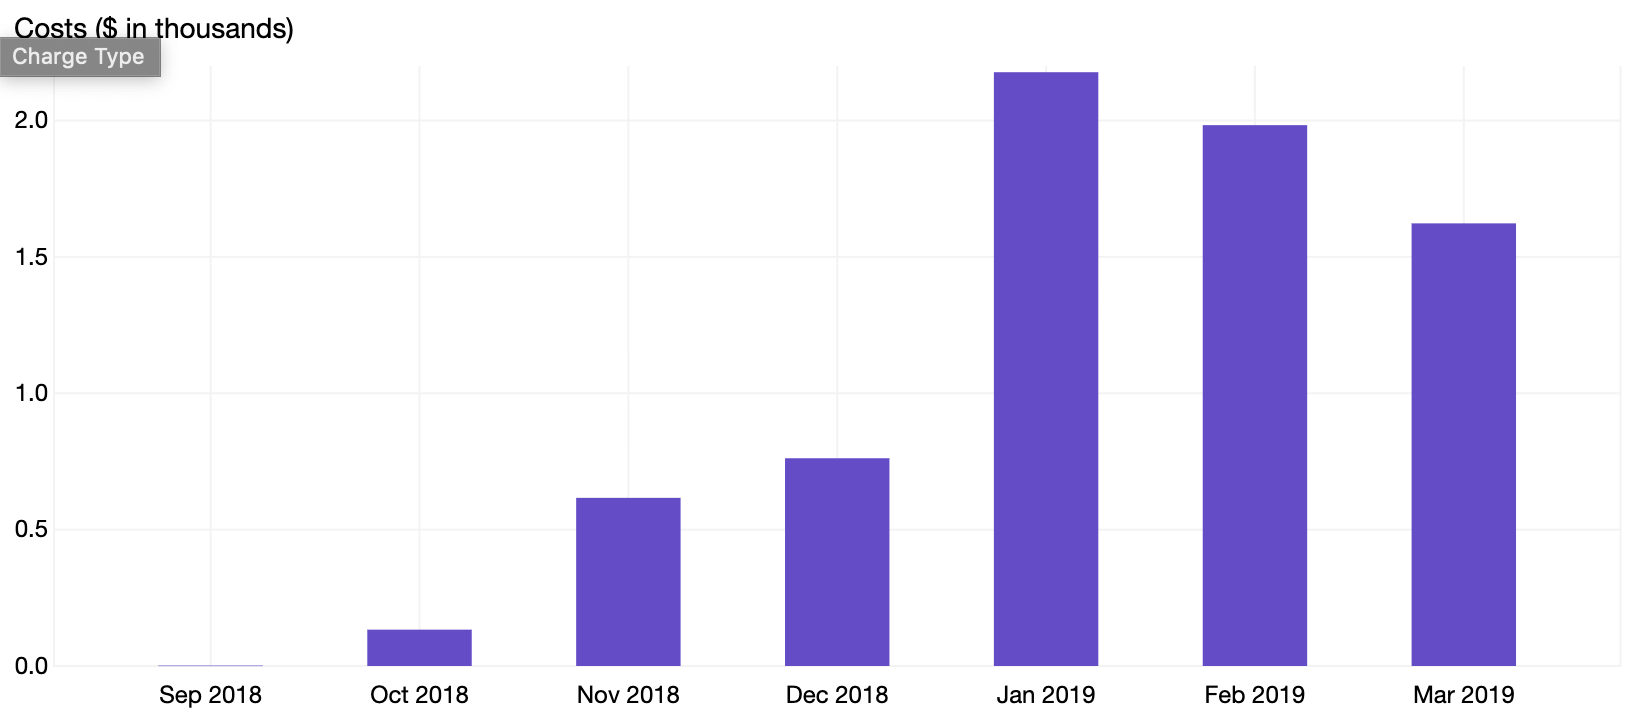
\includegraphics[width=\textwidth]{images/aws-metrics/throughmar/total.png}
\caption{AWS Total Costs\label{fg:awstotal}}
\end{figure}
\begin{figure}[!hbtp]
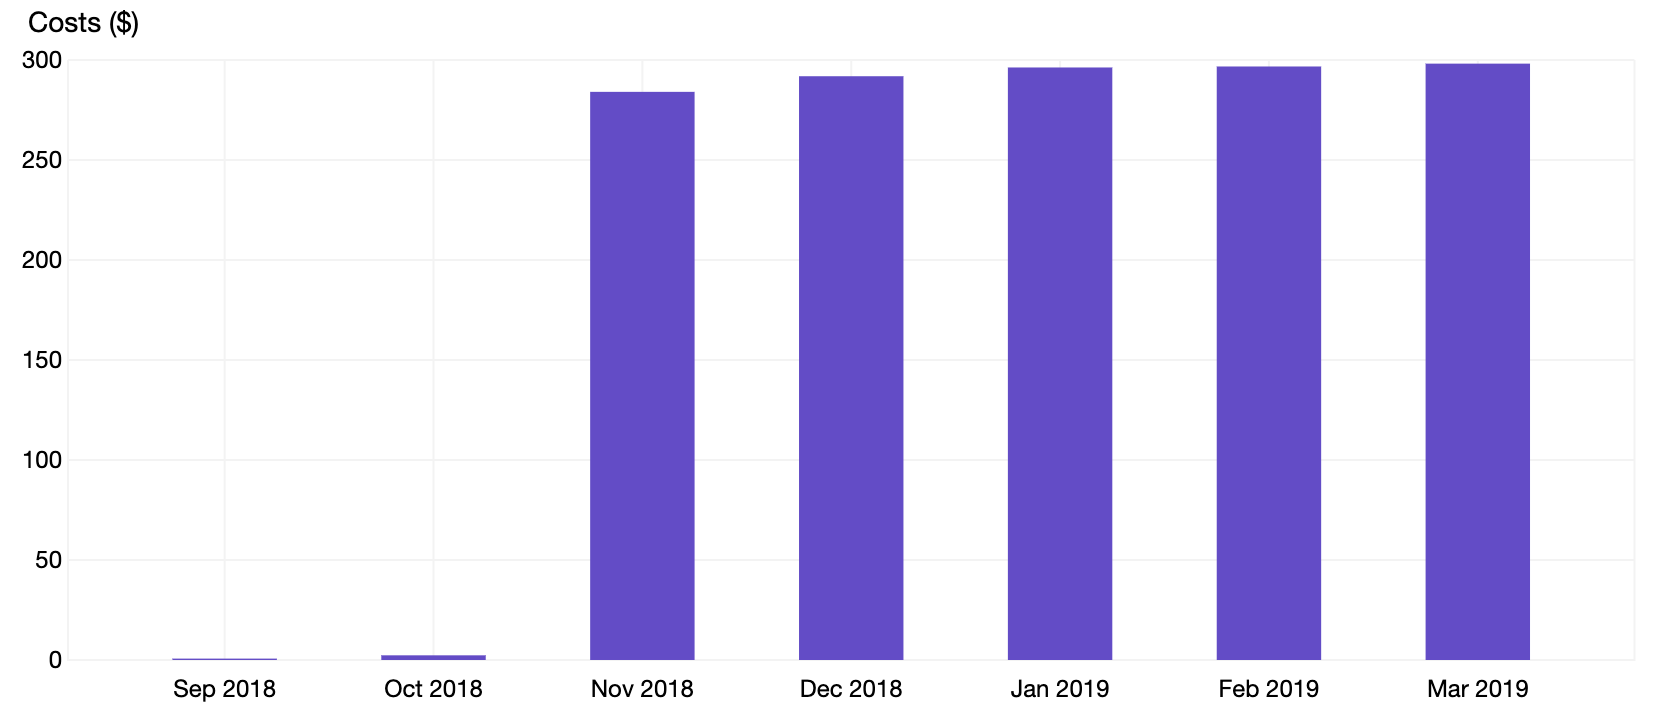
\includegraphics[width=\textwidth]{images/aws-metrics/throughmar/s3.png}
\caption{AWS S3 monthly costs. The main driver is 13.3\,TB for the Healthy Markets project\label{fg:awss3}}
\end{figure}


\section{Local UVA HPC usage}
The Open Data Lab assists researchers in getting access to the local UVA HPC resources. For many of the tasks our users have there is no direct charge from local HPC and we do not track this usage. For more sustained efforts we do track the usage broken down by allocation.

The undergraduate UVA Machine Learning Club used up their entire initial allocation of 5,000\,SUs. They have been issued a new allocation of 100,000\,SUs. Some of their results can be seen in section~\ref{sec:mlc}

The graduate UVA Machine Learning Club has used over half of their intial allocation. They have 3,335\,SUs used and 1,665\,SUs remaining.

\section{Sustained Support}
Many researchers are interested in using the Open Data Lab for continued hosting of their data sets to satisfy data management plan requirements of funding agencies. For example a federal agency that requires a seven year data commitment. In order for the open data lab to support this effort a budget model, at least in part, must provide for multi year sustained support.

\section{Funding Sources}
The ODL is funded by the DSI. The support for the Healthy Markets project is fronted by the ODL and then  cost transferred from the ODL PTAO to the HM PTAO.













%\chapter{publications}

\end{document}




% I view ‘open’ broadly. Open means: accessible, useable, and responsible. Whatever the context, be it data, methods, education, or even lavatories, accessibility and usability are essential for openness. However just as essential is the responsibility. That may take the form of ethical responsibility, scientific responsibility, financial responsibility, educational responsibility, and the list goes on. By necessity this means, open does not imply free. The burden of responsibility lies both with the producer and the consumer. Which means that open means community. Open means culture. Both of these states are not free but they are empowering and well worth the price of openness.
